\documentclass[11pt]{article}

% ACL review layout: anonymous author block, page numbers, and line numbers.
% Change "review" to "final" only for the final non-anonymous copy.
\usepackage[review]{acl}

% This course report keeps review-mode line numbers but is not anonymous.
\makeatletter
\acl@anonymizefalse{}
\makeatother

% Standard packages.
\usepackage{times}
\usepackage{latexsym}
\usepackage[T1]{fontenc}
\usepackage[utf8]{inputenc}
\usepackage{microtype}
\usepackage{inconsolata}
\usepackage{graphicx}
\usepackage{booktabs}
\usepackage{array}
\usepackage{float}
\usepackage{amsmath}
\usepackage{url}

% Keeps headings independently breakable while this file is still an
% empty scaffold. Remove each call as its section receives prose.
\newcommand{\scaffoldspace}{\noindent\mbox{\strut}\par}
\newcommand{\dialogueturn}[2]{\noindent\textbf{#1:} #2\par\smallskip}

% Final-report constraints:
% - Maximum 2,000 words, excluding abstract, references, figures,
%   equations, and appendices.
% - Emphasize the author's own experiments, observations, and analysis.
% - Include repository paths.
% - Put example dialogues and the final LLM prompt in the appendix.

\title{An Experimental Study of Task-Oriented Dialogue Systems}

\author{Ahmed Moustafa \\
  Matriculation Number: 3968514 \\
  Supervisor: Dr.\ Nurul Fithria Lubis \\
  Heinrich Heine University D\"usseldorf}
\date{}

\begin{document}
\maketitle

\begin{abstract}
Task-oriented spoken dialogue systems help users complete goals, such as
finding a restaurant or arranging a hotel stay, through natural-language
interaction. A complete system must represent the user's words, identify
intents and slot values, maintain the dialogue state, choose the next action,
and generate a suitable response. This report studies these decisions through
six connected experiments, from word embeddings and a modular ConvLab3
pipeline to learned language understanding, dialogue state tracking,
reinforcement learning, and LLM-based agents. The emphasis is on the
implementation choices, observed results, and limitations of each approach.
\end{abstract}

\section{Word Embeddings}\label{sec:embeddings}
One-hot vectors treat every word as an independent symbol and do not express
similarity between related words. Dense word embeddings instead learn compact
vectors from context. This lets a dialogue model share evidence between related
slot values, such as different locations or price ranges. In Exercise~1, I
studied Word2Vec \citep{mikolov-etal-2013-distributed}, FastText
\citep{bojanowski-etal-2017-enriching}, and a small custom Skip-Gram model. I
first trained Word2Vec from scratch on the general-domain \textit{text8}
corpus. The domain-specific models used the provided set of 1,364 restaurant
utterances from the second Dialogue State Tracking Challenge (DSTC2)
\citep{henderson-etal-2014-second}.

The \textit{text8} model produced 100-dimensional vectors for 71,290 word
types. Its nearest neighbours for \textit{apple} were mainly technology and
company terms, as shown in Table~\ref{tab:word-embedding-results}. In a
candidate comparison, \textit{fruit} was selected when no technology term was
present, but \textit{computer} was selected after it was added. This illustrates
a limitation of static embeddings: different senses of a word share one
vector, so the most common corpus context can dominate the representation.

\begin{table}[t]
  \centering
  \small
  \begin{tabular}{@{}
    >{\raggedright\arraybackslash}p{0.22\columnwidth}
    >{\raggedright\arraybackslash}p{0.21\columnwidth}
    >{\raggedright\arraybackslash}p{0.45\columnwidth}@{}}
    \toprule
    \textbf{Model} & \textbf{Query} & \textbf{Nearest neighbours} \\
    \midrule
    \textit{text8} W2V & \textit{apple} & macintosh (.792), intel (.716), ibm (.715) \\
    \addlinespace[2pt]
    DSTC2 W2V & \textit{west} & south (.897), east (.864), north (.831) \\
    \addlinespace[2pt]
    DSTC2 W2V & \textit{moderate} & expensive (.544), cheap (.521) \\
    \addlinespace[2pt]
    FastText & \textit{inexpensive} & expensive (.991), give (.590), moderate (.547) \\
    \addlinespace[2pt]
    Custom Skip-Gram & \textit{cheap} & moderate, expensive, price \\
    \bottomrule
  \end{tabular}
  \caption{Selected nearest neighbours from the saved Exercise~1 run. W2V
  abbreviates Word2Vec. Parentheses show cosine similarity; the custom model
  did not save similarity scores.}
  \label{tab:word-embedding-results}
\end{table}

On DSTC2, the Gensim Word2Vec model used the default CBOW architecture with 300
dimensions, a context window of 3, a minimum count of 1, and 1,000 epochs. It
grouped location words and price values, although the similarity between
opposite price values shows that related context does not imply equal meaning.
FastText could also construct a vector for the unseen word
\textit{inexpensive} from character subwords.
However, it ranked the antonym \textit{expensive} first with a similarity of
.991. Subword information therefore improves coverage, but spelling overlap
can be risky when a dialogue system interprets user preferences.

Finally, the custom 100-dimensional, full-softmax Skip-Gram model used a
window of 5 and was trained for 100 epochs. Its saved mean batch loss fell from
4.233 at epoch 0 to 3.361 at epoch 90, with most of the improvement occurring
by epoch 10. Its nearest neighbours formed useful groups for price, location,
and cuisine. These results are qualitative: the notebook contains one saved
run without fixed random seeds or a held-out evaluation. I also excluded its
sentence-similarity values because that helper averaged characters rather than
tokenized words.

\section{Toolkit and Corpora}\label{sec:toolkit}
Task-oriented systems predict structured actions that help a user reach a
specific goal. In a modular pipeline, natural language understanding (NLU)
maps an utterance to dialogue acts, dialogue state tracking (DST) updates the
current slot values, the policy selects a system act using this state and the
database result, and natural language generation (NLG) realizes the act as
text. ConvLab3 standardizes the interfaces between these modules and uses
\texttt{PipelineAgent} to execute them in sequence \citep{zhu-etal-2023-convlab}.
This design makes individual components easy to replace, although an error in
an early module can propagate through the complete pipeline.

\subsection{Simple MultiWOZ 2.1 and the Unified Format}
Simple MultiWOZ 2.1 is the hotel-and-restaurant subset of MultiWOZ 2.1
\citep{eric-etal-2020-multiwoz}. The local unified archive contains 2,503
dialogues: 2,162 for training, 164 for validation, and 177 for testing.
General-domain acts represent functions such as greeting, thanking, and
ending a conversation.

The unified format consists of dialogue records, an ontology, and a database
interface. The ontology defines domains, slots, possible categorical values,
intents, dialogue acts, and the state structure. Each dialogue contains a user
goal and turns labelled with the speaker, utterance, and dialogue acts; the
format can also attach user states, database results, and booked entities.
Dialogue acts may be categorical
intent--slot--value labels, non-categorical values linked to spans in the
utterance, or binary acts without values. These annotations support all four
pipeline modules: utterances supervise NLU acts, dialogue histories supervise
states, states and database results supervise policy actions, and system acts
are paired with responses for NLG.

\subsection{Baseline ConvLab3 Pipeline}
I completed the supplied \texttt{interact.py} baseline. The system agent used
a \texttt{BERTNLU} checkpoint trained on user turns, rule-based state tracking,
the supplied maximum-likelihood policy, and template-based NLG. I disabled
manual entity-name features to match the saved policy's state-vector
dimensions. \texttt{PipelineAgent} connected the modules, while the
command-line loop initialized each session, limited interaction to 40 turns,
and stopped when the user entered \texttt{bye}.

In the recorded interaction in Appendix~\ref{app:dialogues}, the system moved
from a restaurant request to a hotel request and returned relevant entities.
However, it recommended an expensive restaurant after the user requested a
cheap one, produced awkward template phrases, and did not confirm either
booking request. This shows that a plausible response is not sufficient for
reliable goal completion. Improvements should validate policy actions against
the tracked constraints and database results, represent booking status
explicitly, request clarification when information is uncertain, and refine
the response templates. More policy training on constraint changes and
multi-domain booking dialogues would also target the observed failures.

% This is the most important section. Focus on the author's measured results,
% concrete choices, and explanations of which factors changed performance.

\section{Natural Language Understanding with BERTNLU}\label{sec:nlu}
\subsection{Task and Model}
In Exercise~3, I completed and trained ConvLab3's BERTNLU model
\citep{devlin-etal-2019-bert,zhu-etal-2023-convlab}. Preprocessing produced
11,806 training, 1,007 validation, and 1,064 test user turns, with 70 intent
labels and 17 BIO slot tags. Each sample supplies WordPiece identifiers and
attention masks for the current utterance and up to three earlier utterances.
Categorical and binary dialogue acts become a multi-label intent target, while
non-categorical values are represented by token-level BIO tags. The model
outputs 70 intent logits per utterance and 17 slot logits per token. Training
minimizes the sum of weighted binary cross-entropy for intents and
cross-entropy for slot tags.

\subsection{Training Configuration}
The configuration controls the encoder and tokenizer, context use, fine-tuning,
hidden size, dropout, batch size, learning rate, sequence limit, optimizer,
seed, device, and training length. I used the supplied
\texttt{prajjwal1/bert-mini} encoder with the
\texttt{bert-base-uncased} tokenizer because it was small enough for local
training while retaining contextual representations. I fine-tuned the encoder
and context branch for 5,000 updates on a laptop GPU, using batch size 64,
learning rate $10^{-4}$, dropout 0.1, a 40-token utterance limit, three context
turns, and seed 2019. Validation was run every 500 updates, and the checkpoint
with the highest validation F1 was retained.

\subsection{Evaluation and Analysis}
Table~\ref{tab:bertnlu-results} reports corpus-level dialogue-act scores from
the completed evaluator. Exact match is stricter: every predicted act for an
utterance must equal its reference set. Test F1 was 0.43 points above
validation F1, and exact match rose by 1.23 points, so there was no observed
generalization drop between these splits.

\begin{table}[H]
  \centering
  \small
  \setlength{\tabcolsep}{4pt}
  \begin{tabular}{@{}lrrrr@{}}
    \toprule
    \textbf{Split} & \textbf{P} & \textbf{R} & \textbf{F1} & \textbf{Exact} \\
    \midrule
    Validation & 84.79 & 89.46 & 87.06 & 73.49 \\
    Test       & 85.76 & 89.30 & 87.49 & 74.72 \\
    \bottomrule
  \end{tabular}
  \caption{BERTNLU dialogue-act results in percent. P and R denote precision
  and recall; Exact is utterance-level exact-match accuracy.}
  \label{tab:bertnlu-results}
\end{table}

\begin{figure}[H]
  \centering
  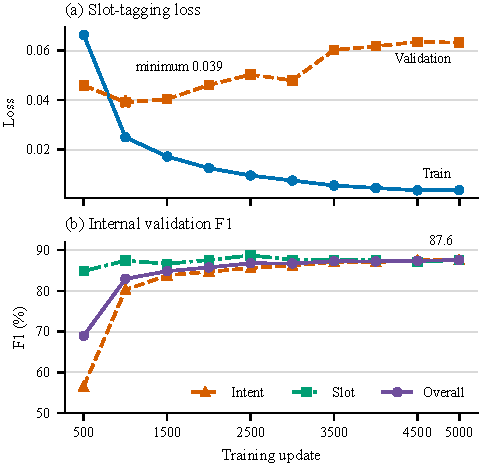
\includegraphics[width=\columnwidth]{figures/bertnlu_learning_curves.pdf}
  \caption{BERTNLU learning dynamics at 500-step checkpoints. The curves are
  unsmoothed; training loss averages the preceding 500 batches, while
  validation loss covers the complete split.}
  \label{fig:bertnlu-learning}
\end{figure}

\begin{figure}[H]
  \centering
  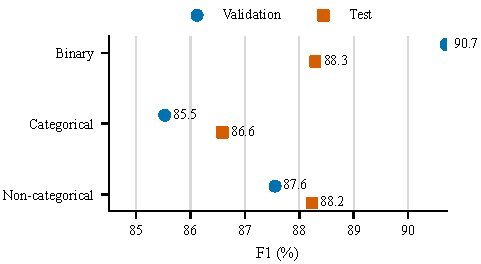
\includegraphics[width=\columnwidth]{figures/bertnlu_act_type_f1.pdf}
  \caption{Standardized validation and test F1 by dialogue-act type.}
  \label{fig:bertnlu-act-types}
\end{figure}

Recall exceeded precision on both splits. Figure~\ref{fig:bertnlu-act-types}
shows that categorical acts were consistently weakest. Their test F1 was
86.13, compared with 87.85 for non-categorical spans and 89.05 for binary
acts. Errors included missing an area expressed indirectly through context,
dropping the multiword value \textit{Eastern European}, and confusing two-
and three-star categories.

Figure~\ref{fig:bertnlu-learning} shows a different pattern for loss and F1.
Training slot loss fell from 0.0679 at step 500 to 0.0036 at step 5,000,
whereas validation slot loss reached its minimum at step 1,000 and then rose
from 0.0395 to 0.0632. Internal validation F1 nevertheless increased from
68.42 to 87.09, so F1-based checkpoint selection retained the final model.
The loss divergence suggests mild overfitting. Other limitations are the
single seeded run, fixed three-turn context, a fixed intent threshold, and
dependence on exact span annotations; preprocessing skipped one malformed
restaurant span. Useful next steps are multi-seed evaluation, threshold tuning,
early stopping, a constrained BIO decoder, and correction of noisy spans.

\section{Dialogue State Tracking with TripPy}\label{sec:dst}
\scaffoldspace{}

\subsection{Architecture, Inputs, and Objective}
\scaffoldspace{}
% Exercise 4:
% Explain TripPy's class, span, and refer gates; model input/output;
% auxiliary features and their intuition; and the weighted multi-task loss.

\subsection{Training Dynamics}
\scaffoldspace{}
% Required figure:
% plot training and validation loss for the full model.
% Explain the trend rather than merely describing the curves.

\subsection{Ablation Study and Analysis}
\scaffoldspace{}
% Required table:
% rows = full features, no auxiliary features, no history or auxiliary
% features; columns = validation JGA and test JGA.
% Identify which input choice mattered most and explain why.

\section{Dialogue Policy with PPO}\label{sec:policy}
\scaffoldspace{}

\subsection{PPO Setup and Policy Variants}
\scaffoldspace{}
% Exercise 5:
% Briefly introduce semantic-level PPO, the rule-based user simulator,
% generalized advantage estimation, and the clipped objective.
% Describe the two policy configurations and the selected hyperparameter
% difference, including the initialization policy.

\subsection{RL Training Results}
\scaffoldspace{}
% Required figure/table:
% compare the two policies using success rate, average actions, reward,
% or other relevant TensorBoard measures.
% Explain how the selected hyperparameter affected learning and performance.

\subsection{Interaction Quality}
\scaffoldspace{}
% Compare measured RL performance with observed conversations and with the
% Exercise 2 baseline policy. Explain agreements or discrepancies.
% Put full dialogue transcripts in Appendix~\ref{app:dialogues}.

\section{Agentic Task-Oriented Dialogue}\label{sec:agentic}
\scaffoldspace{}

\subsection{Free-Form Web-Enabled LLM}
\scaffoldspace{}
% Exercise 6, Task 2:
% Describe the model/interface, goal-completion outcome, and at least two
% boundary probes. Analyze naturalness, flexibility, controllability,
% booking guarantees, safeguards, and provider-ranking behavior.

\subsection{Structured Modular Prompting}
\scaffoldspace{}
% Exercise 6, Task 3:
% Explain the refined NLU--DST--Policy--NLG prompt, use of the supplied hotel
% database, explicit state tracking, intermediate representations, and
% multi-turn goal completion. Put the complete prompt in Appendix~\ref{app:prompt}.

\subsection{Comparison and Deployment Risks}
\scaffoldspace{}
% Compare the modular baseline, free-form LLM, and structured-prompt LLM.
% Discuss goal completion, naturalness, flexibility, controllability,
% shortcomings, whether prompting can replace the modular system, and risks
% of deploying a web-enabled LLM as a customer-service front end.

\section{Conclusion}\label{sec:conclusion}
\scaffoldspace{}
% Summarize the strongest findings across Exercises 1--6.
% Reflect on what worked, the main challenges, and concrete improvements.
% Do not introduce new results.

% Keep the core method references visible while the report body is a scaffold.
% Remove this \nocite command once every work is cited in the prose.
\nocite{mikolov-etal-2013-distributed,
  bojanowski-etal-2017-enriching,
  devlin-etal-2019-bert,
  eric-etal-2020-multiwoz,
  zhu-etal-2023-convlab,
  heck-etal-2020-trippy,
  schulman-etal-2017-ppo,
  schulman-etal-2016-gae}
\bibliography{references}

\appendix

\section{Implementation and Reproducibility}\label{app:implementation}
The exercise implementations are collected in the
\href{https://github.com/x4ahmed/spoken-dialogue-systems}
{\textit{spoken-dialogue-systems} GitHub repository}. The separate HHU GitLab
course forks are
\href{https://git.hhu.de/fiw89rif/convlab3}{ConvLab3} and
\href{https://git.hhu.de/fiw89rif/trippy}{TripPy}. The completed Exercise~2
pipeline is available in the
\href{https://github.com/x4ahmed/spoken-dialogue-systems/blob/main/convlab3/examples/agent_examples/interact.py}
{ConvLab3 interaction script}. Exercise~3 is represented by the
\href{https://github.com/x4ahmed/spoken-dialogue-systems/blob/main/convlab3/convlab/nlu/jointBERT/train.py}
{training script},
\href{https://github.com/x4ahmed/spoken-dialogue-systems/blob/main/convlab3/convlab/nlu/evaluate_unified_datasets.py}
{evaluator}, and
\href{https://github.com/x4ahmed/spoken-dialogue-systems/blob/main/convlab3/convlab/nlu/jointBERT/unified_datasets/configs/simplemultiwoz21_user_context3_exercise3.json}
{run configuration}. It was executed on Windows in the Conda base environment
with Python 3.13.5, PyTorch 2.8.0, Transformers 4.49.0, and an NVIDIA GeForce
RTX 3050 Laptop GPU, using seed 2019. The Exercise~3 figures can be regenerated
from the checked-in metric extracts with the
\href{https://github.com/x4ahmed/spoken-dialogue-systems/blob/main/Report/scripts/plot_bertnlu_evaluation.py}
{plotting script}.

\section{Example Dialogues}\label{app:dialogues}
\scaffoldspace{}
% Dialogue examples are excluded from the word limit.

\subsection{Baseline ConvLab3 Pipeline}
The user goal was to find a cheap restaurant in the south, find a hotel in the
same area with free parking, and book both places. The transcript is reproduced
from the saved Exercise~2 interaction, with speaker labels and punctuation
normalized for readability.

\begingroup
\small
\dialogueturn{System}{Hello, how can I help you?}
\dialogueturn{User}{I am looking for a restaurant in the south part of town.}
\dialogueturn{System}{It is located in the south. There are 9 available
restaurants. That is a chinese restaurant. They are in the expensive price
range. What type of food would you like?}
\dialogueturn{User}{I want cheap food.}
\dialogueturn{System}{Would you like to try the good luck chinese food
takeaway? It is located in the south. I have 9 options for you. It is chinese
food. They are in the expensive price range. I would suggest the good luck
chinese food takeaway.}
\dialogueturn{User}{Can you also find me a hotel in the south?}
\dialogueturn{System}{There are 1 of those.}
\dialogueturn{User}{Does it have free parking?}
\dialogueturn{System}{How about the lensfield hotel? They are located in the
south. We have 1 such places. It is a hotel.}
\dialogueturn{User}{Book a table at the chinese food takeaway restaurant at
20:00 today and one room at lensfield hotel today at 22:00.}
\dialogueturn{System}{Does the the lensfield hotel work? It is located at
53--57 lensfield road. It is indeed in the south. The wifi is included. This is
an expensive hotel. It is a hotel. Is there anything else I can help you with
today?}
\dialogueturn{User}{Yes, book a room.}
\dialogueturn{System}{You are welcome. Is there anything else I can help you
with today?}
\dialogueturn{User}{Bye.}
\dialogueturn{System}{Goodbye!}
\endgroup

\subsection{PPO Dialogue Policies}
\scaffoldspace{}
% Exercise 5 interaction transcript(s), including the comparison with the
% Exercise 2 baseline.

\subsection{Free-Form LLM and Boundary Probes}
\scaffoldspace{}
% Exercise 6 Task 2 transcript and at least two probe exchanges.

\subsection{Structured-Prompt LLM}
\scaffoldspace{}
% Exercise 6 Task 3 multi-turn transcript with intermediate NLU, DST,
% policy, API/database, and NLG representations.

\section{Final Structured Prompt}\label{app:prompt}
\scaffoldspace{}
% Paste the complete final Exercise 6 prompt, including the database or a
% clear description of how it is supplied, the initial state, module output
% schema, constraints, and first user turn.

\end{document}
